\section{Single Square Echo: Cancellation and Spectroscopic Response}
\label{sec:square-echo-comparison}

\subsection{Exact two-level response}

To separate resonant cancellation from the role of the envelope, consider a
square pulse of total duration $L$, with drive $+\Omega_0$ for the first half
and $-\Omega_0$ for the second. The angular detuning $\Delta$ is unchanged by
the phase reversal. In the unitary two-level model,
\begin{equation}
    H_\pm/\hbar=\tfrac12(\Delta\sigma_z\pm\Omega_0\sigma_x),
    \qquad q=\sqrt{\Omega_0^2+\Delta^2}.
\end{equation}
With $\theta=qL/4$, each half-pulse has propagator
\begin{equation}
    U_\pm=\cos\theta\,\mathbb I
      -i\sin\theta\,\frac{\Delta\sigma_z\pm\Omega_0\sigma_x}{q}.
\end{equation}
The complete propagator is $U=U_-U_+$. Multiplication gives
\begin{equation}
    \begin{split}
    U={}&\left[\cos^2\theta-
      \frac{\Delta^2-\Omega_0^2}{q^2}\sin^2\theta\right]\mathbb I\\
      &-i\frac{2\Delta}{q}\sin\theta\cos\theta\,\sigma_z
       -i\frac{2\Omega_0\Delta}{q^2}\sin^2\theta\,\sigma_y.
    \end{split}
\end{equation}
Only the $\sigma_y$ term transfers population between the two bare states.
Starting in the ground state therefore gives
\begin{equation}
    P_e^{\mathrm{sq}}(\Delta)=
      \frac{4\Omega_0^2\Delta^2}{(\Omega_0^2+\Delta^2)^2}
      \sin^4\!\left(\frac{L}{4}\sqrt{\Omega_0^2+\Delta^2}\right).
    \label{eq:square-echo-exact}
\end{equation}
At resonance $U=\mathbb I$ for every drive amplitude, just as for the
root-Lorentzian echo. However, at fixed nonzero $\Omega_0$ and $L$, the
small-detuning expansion is
\begin{equation}
    P_e^{\mathrm{sq}}(\Delta)=
      \frac{4\Delta^2}{\Omega_0^2}
      \sin^4\!\left(\frac{\Omega_0 L}{4}\right)
      +O\!\left[(\Delta/\Omega_0)^4\right].
    \label{eq:square-echo-small-detuning}
\end{equation}
More generally, Eq.~\eqref{eq:square-echo-exact} obeys the bound
\begin{equation}
    0\leq P_e^{\mathrm{sq}}(\Delta)
      \leq\frac{4\Omega_0^2\Delta^2}{(\Omega_0^2+\Delta^2)^2}
      \leq4(\Delta/\Omega_0)^2.
    \label{eq:square-echo-bound}
\end{equation}
Thus, increasing the drive suppresses excitation throughout a fixed
near-resonance window, rather than guaranteeing a visible dip at its center.
The leading curvature also oscillates with pulse area and vanishes when
$\Omega_0 L/4$ is an integer multiple of $\pi$. These are finite-pulse
results; the steady-state Bloch linewidth is not used to describe this echo.

\subsection{Comparison at matched duration and peak drive}

Figure~\ref{fig:square-echo-comparison} compares saved three-level simulations
of the square and root-Lorentzian echoes. Both pulses have $L=20~\mu\mathrm{s}$,
the same peak drive $\Omega_0$, and one abrupt midpoint inversion. The
root-Lorentzian has $n=1/2$ and $c=0.005$. Neither pulse includes DRAG,
polynomial shaping, or an added frequency correction. The Lindblad model
of Sec.~\ref{sec:numerical-model} uses $T_1=43.8~\mu\mathrm{s}$,
$T_2=7.6~\mu\mathrm{s}$, and $\alpha/(2\pi)=-216~\mathrm{MHz}$.
Here $T_2$ specifies a phenomenological Markovian dephasing rate; these
parameters define a controlled numerical comparison, not a fit to Fig.~2.

The displayed drive range is 0.1--$20.05~\mathrm{MHz}$, with spectra sampled
over $\pm0.5~\mathrm{MHz}$ at $2.5~\mathrm{kHz}$ spacing. At
$\Omega_0/(2\pi)=3.05~\mathrm{MHz}$, the total population variation
$V=\max_\Delta P_e-\min_\Delta P_e$ within this window is 0.399 for the
root-Lorentzian echo and 0.00481 for the square echo. At $10.05~\mathrm{MHz}$,
the corresponding values are 0.320 and 0.00199. This finite-window variation
quantifies the observable spectral structure; it is not a sensitivity gain.
Both selected drives maximize the ideal square echo's leading curvature:
each half-pulse rotates through an odd multiple of $\pi$. The comparison
therefore avoids its pulse-area cancellation points.

At strong drive, the square echo becomes nearly flat in the central window, while the
root-Lorentzian retains a pronounced depletion feature with the same duration
and cutoff across drives. Dissipation produces a finite population background,
so the square echo's weak spectral variation does not imply negligible
excitation. The wider frequency view shows structure outside
the central window; the square spectrum is not globally featureless.
Matching duration and peak drive does not match integrated drive energy
or pulse area. At the fixed cutoff used here, the root-Lorentzian's
$\int\Omega(t)^2dt$ is approximately 0.78\% of the square pulse's value.

Square-pulse segments were propagated using exact Lindblad matrix
exponentials. The saved unitary calculations agree with
Eq.~\eqref{eq:square-echo-exact} to $3.8\times10^{-13}$ in population.
Halving the root-Lorentzian integration step from 0.5 to $0.25~\mathrm{ns}$
changes the tested populations by less than $2.5\times10^{-5}$. At the
checked drives through $20.05~\mathrm{MHz}$ and detunings
$-500$, $-100$, 0, 100, and $500~\mathrm{kHz}$, adding a fourth level
changes $P_e$ by at most $3.0\times10^{-5}$ for the root-Lorentzian
and $5.5\times10^{-5}$ for the square echo. These are representative
convergence checks, not a bound for every point of the maps.

This comparison concerns a single inversion at fixed duration. Repeated
rotary-echo sequences can generate frequency-dependent fringes and support
sensing~\cite{aiello_composite_pulse_2013}. Their cycle timing and pulse-area
dependence must be assessed separately. The present result establishes the
role of the shaped envelope in producing a visible central depletion feature;
it does not establish superior sensitivity over optimized repeated echoes.

\begin{figure*}[!tp]
    \centering
    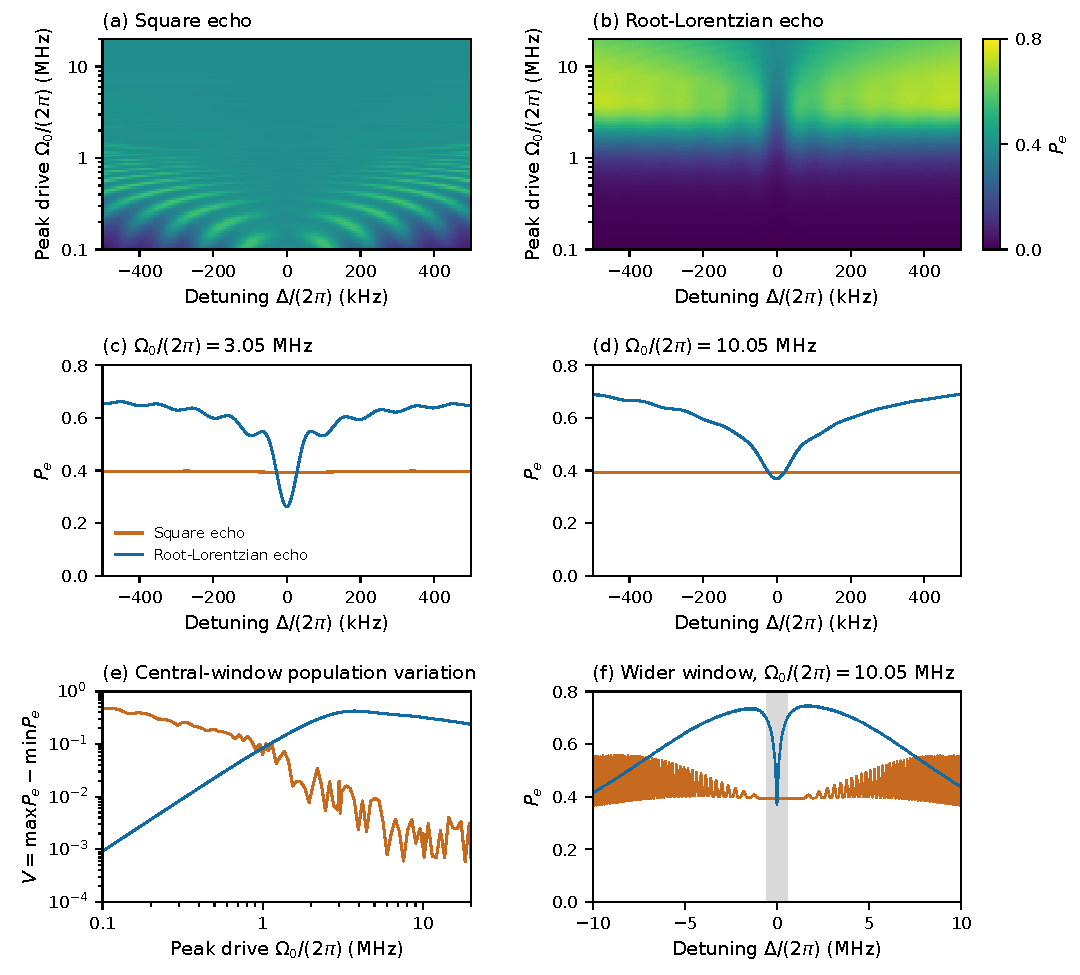
\includegraphics[width=\textwidth]{supplemental/square_echo_comparison.pdf}
    \caption{Single square and root-Lorentzian echoes at equal duration and
    peak drive. All panels use the three-level dissipative model described in
    the text, with one abrupt inversion and no DRAG or polynomial correction.
    (a,b) Final $P_e$ versus detuning and peak drive for the square and
    root-Lorentzian echoes; both maps share the population color scale.
    (c,d) Spectra at 3.05 and $10.05~\mathrm{MHz}$, with identical population
    axes. (e) Population variation $V$ within $\pm0.5~\mathrm{MHz}$ versus
    drive. (f) The $10.05~\mathrm{MHz}$ spectra over a wider detuning range;
    shading marks the central window used in (a)--(e). The square echo's
    weak central response does not imply an absence of structure at larger
    detuning. Curves and maps use saved samples without refitting.}
    \label{fig:square-echo-comparison}
\end{figure*}
